\documentclass[]{iac_class} 

\newcommand{\etalia}{\textit{et al.}}
\newcommand*{\vectornorm}[1]{\left\|#1\right\|}
\newcommand*\rfrac[2]{{{}^{#1}\!/_{#2}}} % running fraction with slash - requires math mode.
\newcommand*\T{\mathsf{T}}

%%%%%%%%%%%%%%%%%%%%%%%%%%%%%%%%%%%%%%%%%%% Other packages %
\usepackage[hidelinks]{hyperref}
\usepackage{wrapfig}
\usepackage{orcidlink}
%\usepackage{amsmath} %,amssymb,amsfonts
\usepackage[inline]{enumitem}   
\newcommand{\comment}[1]{}
\usepackage{blindtext}
%\usepackage{eucal}
\usepackage{lipsum}


%%%%%%%%%%%%%%%%%%%%%%%%%%%%%%%%%%%%%%%%%%% Customization %
% Control header spacing
%\setlength{\headheight}{18pt}
%\addtolength{\topmargin}{-5.75801pt}

% set default enumeration/itemize parameters
\setlist{noitemsep}

%%%%%%%%%%%%%%%%%%%%%%%%%%%%%%%%%%%%%%%%%%% BEGIN DOCUMENT %
\begin{document}

\IACpaperyear{2021}
\IACpapernumber{IAC-21-D2,3,2,xxxxxx}
\IACconference{International Astronautical Congress – IAC 2021, Dubai, United Arab Emirates}
\IAClocation{Dubai, United Arab Emirates}
\IACdate{25-29 October 2021}
\IACcopyrightB{Mr. author 1 and Mr. author 2}

\title{Your paper's title}

\IACauthor{Author 1$^{\orcidlink{0000-0000-0000-0000}}$}{Company location, \normalfont{\texttt{email1@email.com}}}{1}
\IACauthor{Author 2$^{\orcidlink{0000-0000-0000-0000}}$}{Company location, \normalfont{\texttt{email2@email.com}}}{0}

\abstract{%
Your abstract with no new lines.
\\\textbf{Keywords:} Keyword 1, ..., Keyword 6}  % max 6 keywords




\maketitle
\thispagestyle{fancy} % resets proper header/footer

\section{Introduction}
This document is an unofficial \LaTeX model for papers submitted for the International Astronautical Congress. 
\\This template was used to submit \cite{fari2021vector}.
Please observe the conference page for the most updated instruction. 

\section{Styling}\label{sec:styling}
This section offers some template for the most common \LaTeX objects, such as equation, tables and figures.

\subsection{Equations}\label{s_sec:equation} 
\begin{equation}\label{eq:sample_equation}
    W^p=m_pg\left[\begin{matrix}
-s_{\theta_p}\\s_{\phi_p}c_{\theta_p}\\c_{\phi_p}c_{\theta_p}
\end{matrix} \right]
\end{equation}
Equations can be referenced as: ``Eq.~\ref{eq:sample_equation} represents ... ''.




\subsection{Tables}

Tables can be designed as shown in Table~\ref{tab:model_coefficients}.

\begin{table}[t]
\centering
\begin{tabular}{lc|lc}
\textbf{Param.} & \textbf{Value}       & \textbf{Param.} & \textbf{Value}         \\ \hline
$m_p$                & 13                   & $m_b$                & 135                    \\
a                    & 1                    & b                    & 7                      \\
$c$                  & 3                    & $t$                  & 3                      \\
$S_b$                & 0.500                  & $S_p$                & 21                     \\
$\|X_{cb}\|$         & 0.500                  & $\|X_{cp}\|$         & 7.500                    \\
$I_b$                & diag(5.620)           & $I_p(1,1)$          & 53.180 \\
$I_p(2,2)$          &  9.840                 & $I_p(3,3)$          & 62.830\\
$C_{{L,p}_0}$            & 0.400                  & $C_{{L,p}_\alpha}$            &  2                      \\
$C_{{D,p}_0}$            &  0.150                 & $C_{{D,p}_\alpha}$    & 1                       \\
$C_{{D,b}_0}$            &  0.150                 & $C_{{D,b}_\alpha}$    & 1                       \\
$C_{l_p}$            &  -0.100                & $C_{l_\phi}$       &   -0.050                     \\
$C_{m_q}$            & -2                   & $C_{m_0}$          &  0.018                    \\
$C_{n_r}$            & -0.070              & $C_{m_\alpha}$       & -0.200                \\
$C_{L_{\delta_a}}$   & 1\texttt{e-4}      & $C_{L_{\delta_s}}$   &  0.210                      \\
$C_{D_{\delta_a}}$   & 1\texttt{e-4}      & $C_{D_{\delta_s}}$   & 0.300                       \\
$C_{l_{\delta_a}}$ &  21\texttt{e-4}      & $C_{n_{\delta_a}}$   & 0.004\\
$k_k$                &   0.350                   & $c_c$          &  4.700       \\\hline
\end{tabular}
\caption{Model parameters (reported in SI units).}
\end{table}\label{tab:model_coefficients}



\subsection{Figures}\label{sec:figures}

Figures can be included as shown in Figure~\ref{fig:VF_straight_line}.

\begin{figure}
\centering
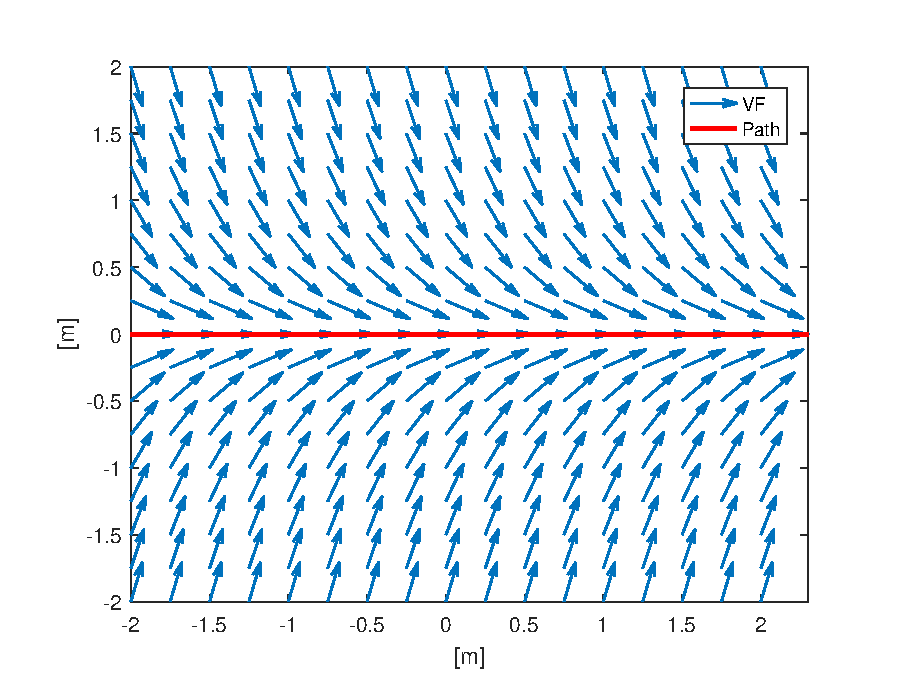
\includegraphics[width = \columnwidth]{images/vf_example.eps}
\caption{Vector field straight-line path-following example.}
\label{fig:VF_straight_line}
\end{figure}







\section{Conclusion and future work}\label{sec:conclusions}
\subsection{Conclusions}\label{ss_sec:first_subsec}
\subsection{Future work}\label{ss_sec:second_subsec}


\bibliographystyle{IEEEtran} 
\bibliography{ref}

\end{document}